\section{Theorie}

In diesem Kapitel wird erläutert wie bei der Dimensionierung eines Stubfilters (Mikrowellenfilter) vorgegangen wird. Um den Leser einen Überblick zu verschaffen, ist in Abb. \ref{fig:Ablauf_Filterdimensionierung} der typische Ablauf zur Dimensionierung von Stubfiltern dargestellt. Der dargestellte Ablauf wird auch für die Realisierung von aktiven, passiven und digitalen Filters verwendet. Der einzige Unterschied ist, dass sich die Schritte in Filter-Realisierung(blau umrandet) unterscheiden.

Ausgangslage für jede Filterdimensionierung ist die Filterspezifikation, welche im Frequenz- oder Zeitbereich vorliegt. Diese Filterspezifikation wird anschliessen mathematisch mit einer Funktion in der s-Ebene (Prototypbereich) beschrieben. Mit einem Synthesetool kann aus der Funktion in der s-Ebene ein Prototypfilter mit konzentrierten Elementen(R,L,C) gefunden werden. Dabei gibt das Synthesetool die Topologie, sowie die Bauteilwerte aus. Liegt kein Synthesetool vor, so müssen Standardfilter (Butterworth, Chebyshev, Bessel,...) verwendet werden, deren Topologie und Bauteilwerte normiert aus einer Tabelle zu entnehmen sind. Bei sehr speziellen Anforderungen an das Filter reichen die Standardfilter aber meist nicht aus um die Filterspezifikationen einzuhalten.

Nach der Synthese liegt nun ein Prototypfilter mit konzentrierten Elementen vor, gesucht ist aber ein Stubfilter, welches aus verteilten Elementen (Leitungen) besteht. Hier kommt die Frequenztransformation von Richards zum Zuge. Richards konnte zeigen, dass sich gleichlange, verlustlose Leitungen (TLSC,TLOC) gleich wie konzentrierte Elemente verhalten, wenn die folgende Transformation für die laplace variable verwendet wird.

s= dhsijdkh

Mit der Frequenztransformation von Richards kann dieses Filter vom Prototypbereich(s-Eben) in den Originalbereich (f-Ebene) transformiert werden. Dadurch werden die konzentrierten Elemente(L,C) in verteilte Elemente (Leitungen) umgewandelt. Dies 
TLSC = ideale, verlustlose Transmission Line im kurzschluss
TLOC = ideale, verlustlse Tranmissin Line im Leerlauf



\newpage

\begin{figure}[h!]
\centering
 	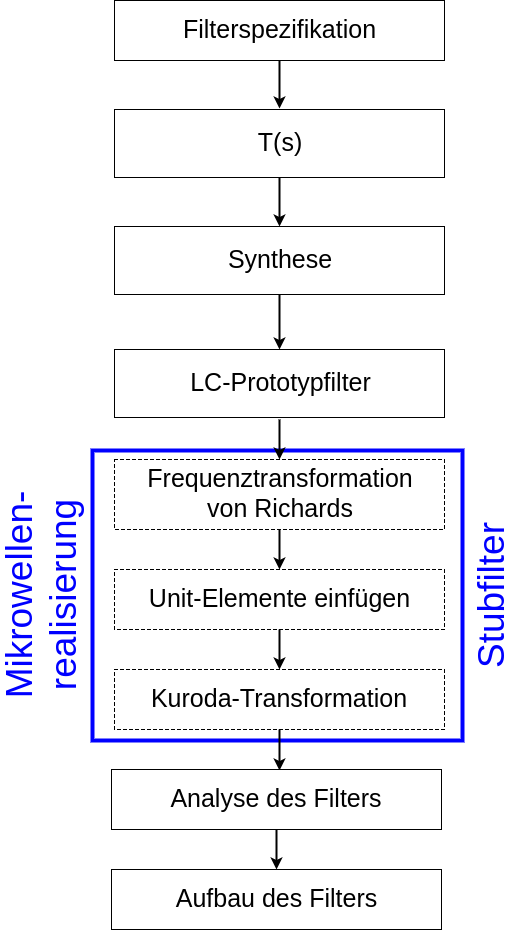
\includegraphics[width=0.5\textwidth]{Ablauf_Filterdimensionierung.png}
 	\caption{Ablauf der Stubfilter-Dimensionierung}
 	\label{fig:Ablauf_Filterdimensionierung}
\end{figure}
